\documentclass[11pt]{article}
\linespread{1}

\usepackage{geometry} % see geometry.pdf on how to lay out the page. There's lots.
\usepackage[utf8]{inputenc}
\usepackage{array}
\usepackage{amsmath,amssymb,latexsym,epic,eepic,epsfig,graphics,psfrag}
\usepackage{amsfonts}
\usepackage{graphicx,float}

\usepackage[danish]{babel}

\usepackage[bottom]{footmisc}

\usepackage{fancyhdr}
\pagestyle{fancy}
\lhead{\small\textit{Detection of human alertness - 01666 Fagprojekt - Anders Hørsted (s082382)}}
\rhead{\thepage}
\chead{}
\lfoot{}\cfoot{}\rfoot{}

\usepackage{pstricks}
\usepackage{pst-node}
\usepackage{wrapfig}
\usepackage{caption}
\usepackage{multirow}
%\usepackage{fouriernc}
%\usepackage[charter]{mathdesign}
\usepackage{lmodern}
\usepackage[normalem]{ulem}
\geometry{a4paper} % or letter or a5paper or ... etc
% \geometry{landscape} % rotated page geometry

\usepackage{url}
\usepackage{natbib}
\renewcommand\bibsection*{}
\bibliographystyle{plain}

\makeatletter
\renewcommand*\env@matrix[1][*\c@MaxMatrixCols c]{%
  \hskip -\arraycolsep
  \let\@ifnextchar\new@ifnextchar
  \array{#1}}
\makeatother

\newcommand\myimp{\quad\Leftrightarrow\quad}
\newcommand\half{\frac{1}{2}}
\newcommand\myvec[1]{\mathbf{#1}}
\newcommand\mymod[1]{\ (\text{mod }#1)}
\newcommand\myreal{\mathbb{R}}
\newcommand\mynatural{\mathbb{N}}
\newcommand\mycomplex{\mathbb{C}}
\newcommand\myint{\text{int}}
\newcommand\norm[1]{||\,#1\,||}
\newcommand\bignorm[1]{\big|\big|\,#1\,\big|\big|}
\newcommand\seq[1]{\big\{#1\big\}}
\newcommand\smallseq[1]{\{#1\}}
\newcommand\smallseqtoinf[1]{\smallseq{#1}_{k=1}^\infty}
\newcommand\lonew{\ell^1_w}
\newcommand\lone{\ell^1}
\newcommand\ltwo{\ell^2(\mynatural)}
\newcommand\ip[2]{\langle#1,#2\rangle}
\newcommand\hilbert[1]{\mathcal{#1}}
\newcommand\uinf{u_{\infty}}
\newcommand\erf{\text{erf\,}}

\usepackage{tabulary}
\newcolumntype{y}{>{\centering\arraybackslash}R}

\title{Homework 1}
\author{01246 Partial differential equations -- 11-09-2011 -- Anders Hørsted (s082382)}
%\author{}
\date{} % delete this line to display the current date

%%% BEGIN DOCUMENT
\begin{document}

\section*{Exercise 1}

A linear, first-order PDE is given by
\begin{equation}\label{eq:ex1}
    u_x + 2yu_y = 0
\end{equation}
Therefore the directional derivative in direction of the vector $v=(1, 2y)^T$ is zero for any solution $u$ of (\ref{eq:ex1}). A solution $u$ will therefore be constant along all curves where
\begin{equation}
    \frac{dy}{dx} = 2y
\end{equation}
In other words any solution $u$ will be constant along curves given by
\begin{equation}\label{eq:char-curves}
    y = Ce^{2x}
\end{equation}
where $C\in\myreal$. 

\subsection*{a)}
Some of these curves are plotted in figure \ref{fig:char-curves}.
\begin{figure}\label{fig:char-curves}
    \centering
    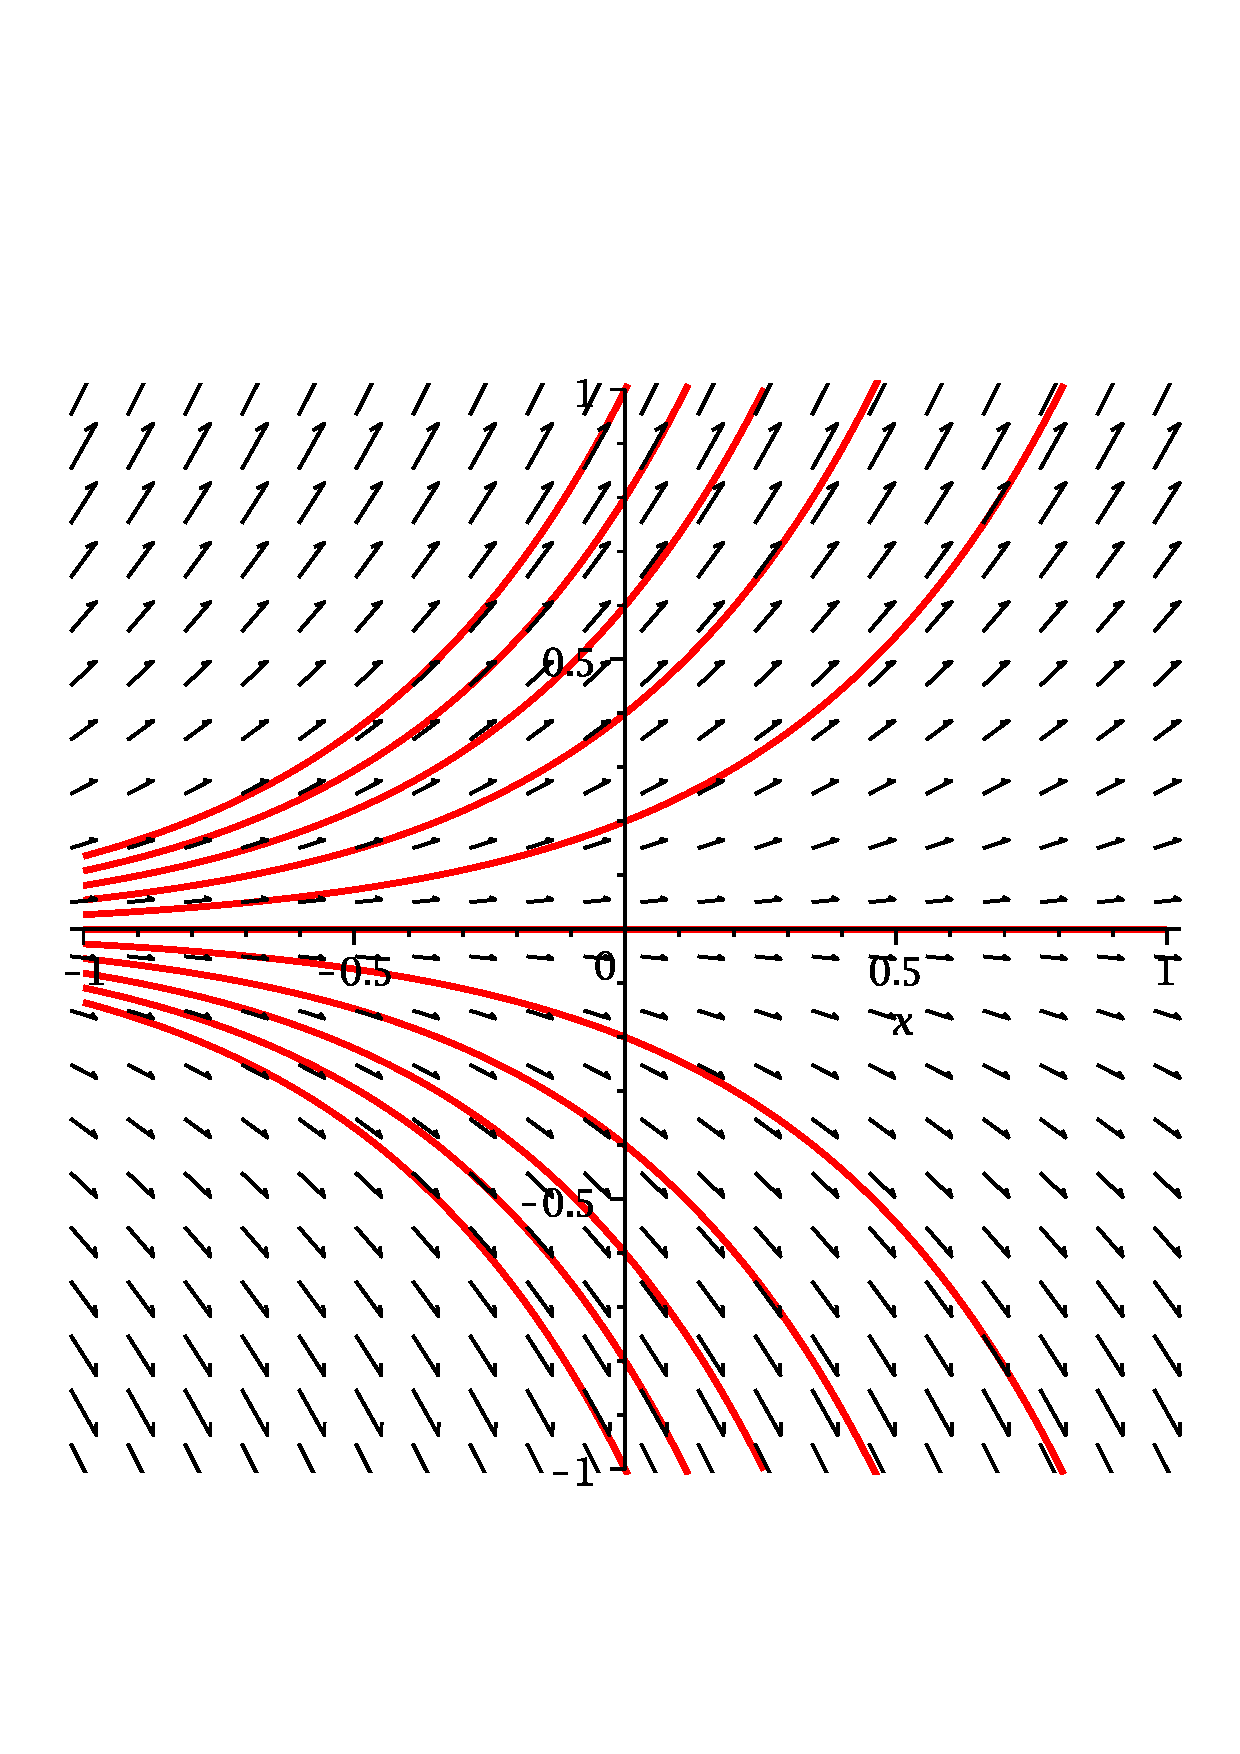
\includegraphics[width=90mm]{characteristic-curves-exercise-1.pdf}
    \caption{Characteristic curves of the PDE given in (\ref{eq:ex1})}
\end{figure}
Along any characteristic line $u$ is constant and the specific value is related to the constant $C$ in (\ref{eq:char-curves}). From (\ref{eq:char-curves}) we get $C=ye^{-2x}$ and therefore
\begin{align}
    u(x, y) &= f(C) \nonumber\\
            &= f(ye^{-2x})\label{eq:ex1-sol}
\end{align}
where $f$ is an arbitrary function of one real variable. From this we conclude that the general solution of (\ref{eq:ex1}) is given by $u(x, t)=f(ye^{-2x})$.

\subsection*{b)}
We now wish to find the solution $u_p$ that satisfies the condition $u(0,y)=y$. By inserting in (\ref{eq:ex1-sol}) we get
\begin{align*}
    u(0, y) &= y \myimp \\
    f(ye^{-2\cdot 0}) &= y \myimp \\
    f(y) &= y
\end{align*}
so $f$ is just the identity function and the particular solution is then given by
\begin{equation}
    u_p(x, y) = ye^{-2x}
\end{equation}

\subsection*{c)}
We now consider the inhomogeneous equation given by
\begin{equation}\label{eq:ex1c-pde}
    u_x + 2yu_y = x
\end{equation}
The general solution to the equation should be found. As the equation is linear the complete general solution will be given as the sum of the general solution to the homogeneous equation and a particular solution to the inhomogeneous equation. The general solution to the homogeneous equation was found in (\ref{eq:ex1-sol}) and therefore only the particular solution $u_p$ to (\ref{eq:ex1c-pde}) needs to be determined. From (\ref{eq:ex1c-pde}) it is directly seen that $u_p(x, y)=\frac{1}{2}x^2$ is a particular solution. The general solution to (\ref{eq:ex1c-pde}) is then given as
\begin{equation}
    u(x, y) = f(ye^{-2x}) + \half x^2
\end{equation}


\section*{Exercise 2}
For $n\in\mynatural$ a second order, inhomogeneous PDE is given by
\begin{gather}\label{eq:hadamard}
    \begin{split}
    \Delta u(x, y) = \frac{\partial^2u}{\partial x^2} + \frac{\partial^2 u}{\partial y^2} = 0, \quad x>0, y\in\myreal \\
    u(0,y) = 0, \quad \frac{\partial u}{\partial x}(0, y) = \frac{1}{n}\sin(ny), \quad y\in\myreal
    \end{split}
\end{gather}

\subsection*{a)}
It is shown that 
\begin{equation}\label{eq:hadamard-sol}
    u_n(x,y) = \frac{1}{n^2}\sin(ny)\sinh(nx)
\end{equation}
solves the problem (\ref{eq:hadamard}). Since $\sinh(0)=0$ it is immediately seen that $u(0,y)=0$. Now the partial derivatives of $u$ is calculated.
\begin{align*}
    u_x(x,y) &= \frac{1}{n}\sin(ny)\cosh(nx) \\
    u_{xx}(x,y) &= \sin(ny)\sinh(nx) \\
    u_y(x,y) &= \frac{1}{n}\cos(ny)\sinh(nx) \\
    u_{yy}(x,y) &= -\sin(ny)\sinh(nx)
\end{align*}
From this it is seen that
\begin{align*}
    u_x(0, y) &= \frac{1}{n}\sin(ny)\cosh(0) \\
              &= \frac{1}{n}\sin(ny)
    \intertext{and}
    u_{xx}+u_{yy} &= \sin(ny)\sinh(nx) - \sin(ny)\sinh(nx) \\
                  &= 0
\end{align*}
and therefore (\ref{eq:hadamard-sol}) solves (\ref{eq:hadamard}).

\subsection*{b)}
It now needs to be shown that the solution (\ref{eq:hadamard-sol}) is unique. First we look at the homogeneous problem related to (\ref{eq:hadamard}). This is just the same problem, with the condition $u_x(0,y)=\frac{1}{n}\sin(ny)$, substituted with $u_x(0,y)=0$. A solution to the homogeneous problem is denoted $\uinf$ and it is assumed that $\uinf$ is independent of $y$. Since $\uinf$ is a solution to the homogeneous problem and independent of $y$ we get
\begin{equation*}
    \frac{\partial^2 \uinf}{\partial x^2} = 0 \quad,\quad \frac{\partial \uinf}{\partial x}(0,y) = 0 \quad,\quad \uinf(0,y) = 0
\end{equation*}
Since $\frac{\partial^2 \uinf}{\partial x^2} = 0$ we have that $\frac{\partial \uinf}{\partial x}$ must be constant, and since $\frac{\partial \uinf}{\partial x}(0,y) = 0$, we conclude that $\frac{\partial \uinf}{\partial x}=0$. Since $\frac{\partial \uinf}{\partial x}=0$ then $\uinf$ must be a constant and since $\uinf(0,y)=0$ we get that $\uinf = 0$. With this result it can now be shown that (\ref{eq:hadamard-sol}) is the unique solution to (\ref{eq:hadamard}). \\
Assume that $u_{n_2}$ is another solution for (\ref{eq:hadamard}). Since the problem is linear $u_0=u_n-u_{n_2}$ is a solution to the homogeneous problem. But from the previous result $u_0=0$ and therefore
\begin{align*}
    u_n - u_{n_2} &= 0 \myimp\\
    u_n &= u_{n_2}
\end{align*}
and so (\ref{eq:hadamard-sol}) is the unique solution of (\ref{eq:hadamard}).

\subsection*{c)}
It now needs to be determined whether (\ref{eq:hadamard}) is a well-posed problem or not. The previous two sections have established both the existence and the uniqueness of (\ref{eq:hadamard}) and only the stability of the problem remains to be examined. For $x=0$ we get
\begin{align*}
    u_n(0,y) &= 0 \\
    &\to 0 \text{ for } n\to\infty
\end{align*}
but for $x>0$
\begin{align*}
    \frac{\sinh(nx)}{n^2} &= \frac{e^{nx} - e^{-nx}}{2n^2} \\
    &\to \infty \text{ for } n\to\infty
\end{align*}
and so 


\section*{Exercise 3}
A solution for the initial value problem for the wave equation
\begin{gather*}
    u_{tt} - 4u_{xx} = 0,\quad x,t\in\myreal \\
    u(x, 0) = 0,\quad u_t(x, 0)=e^{-x^2}, \quad x\in\myreal
\end{gather*}
is found, and the solution is expressed in terms of the error function. Using d'Alembert formula (eq. 2.1.8) with $c=2$, $\phi(x)=0$ and $\psi(x)=e^{-x^2}$, we get
\begin{align*}
    u(x, t) &= \frac{1}{2}(0+0)+\frac{1}{4}\int_{x-2t}^{x+2t}e^{-s^2}\,ds \\
    &= \frac{1}{4}\int_{x-2t}^{x+2t}e^{-s^2}\,ds
\end{align*}
To express the solution in terms of the error function, the sign of $x+2t$ and $x-2t$ as well as the sign of $t$ should be considered. With the help of Maple it turns out that all cases can be expressed in a single expression. That is
\begin{align*}
    u(x, t) &= \frac{1}{4}\int_{x-2t}^{x+2t}e^{-s^2}\,ds \\
    &= \frac{1}{4}\left(\int_{0}^{-x+2t}e^{-s^2}\,ds + \int_{0}^{x+2t}e^{-s^2}\,ds\right)
\end{align*}
The validity of the above can easily be checked for all possible combinations of the sign of $x+2t$, $x-2t$ and $t$. Now the solution can be expressed as
\begin{align*}
    u(x, t) = \frac{\sqrt{\pi}}{8}\left(\erf(-x+2t) + \erf(x+2t)\right)
\end{align*}


\end{document}
